% ============================================================================
% SECTION 4: ENTITY STATE MACHINES & MAIN WORKFLOW ACTIVITY DIAGRAMS
% ============================================================================
\section{Entity State Machine Diagrams and Main Business Workflows}

\subsection{Entity State Machine Diagrams}

To ensure consistency between the Software Design Document and the domain enumerations (com.historytalk.\ab entity.enums), Figures~\ref{fig:stm_01_content_and_account}, \ref{fig:stm_02_assignment_and_token}, and \ref{fig:stm_03_payment_lifecycle} model the finite state machines of the stateful domain lifecycles in HistoryTalk.

\begin{figure}[htbp]
    \centering
    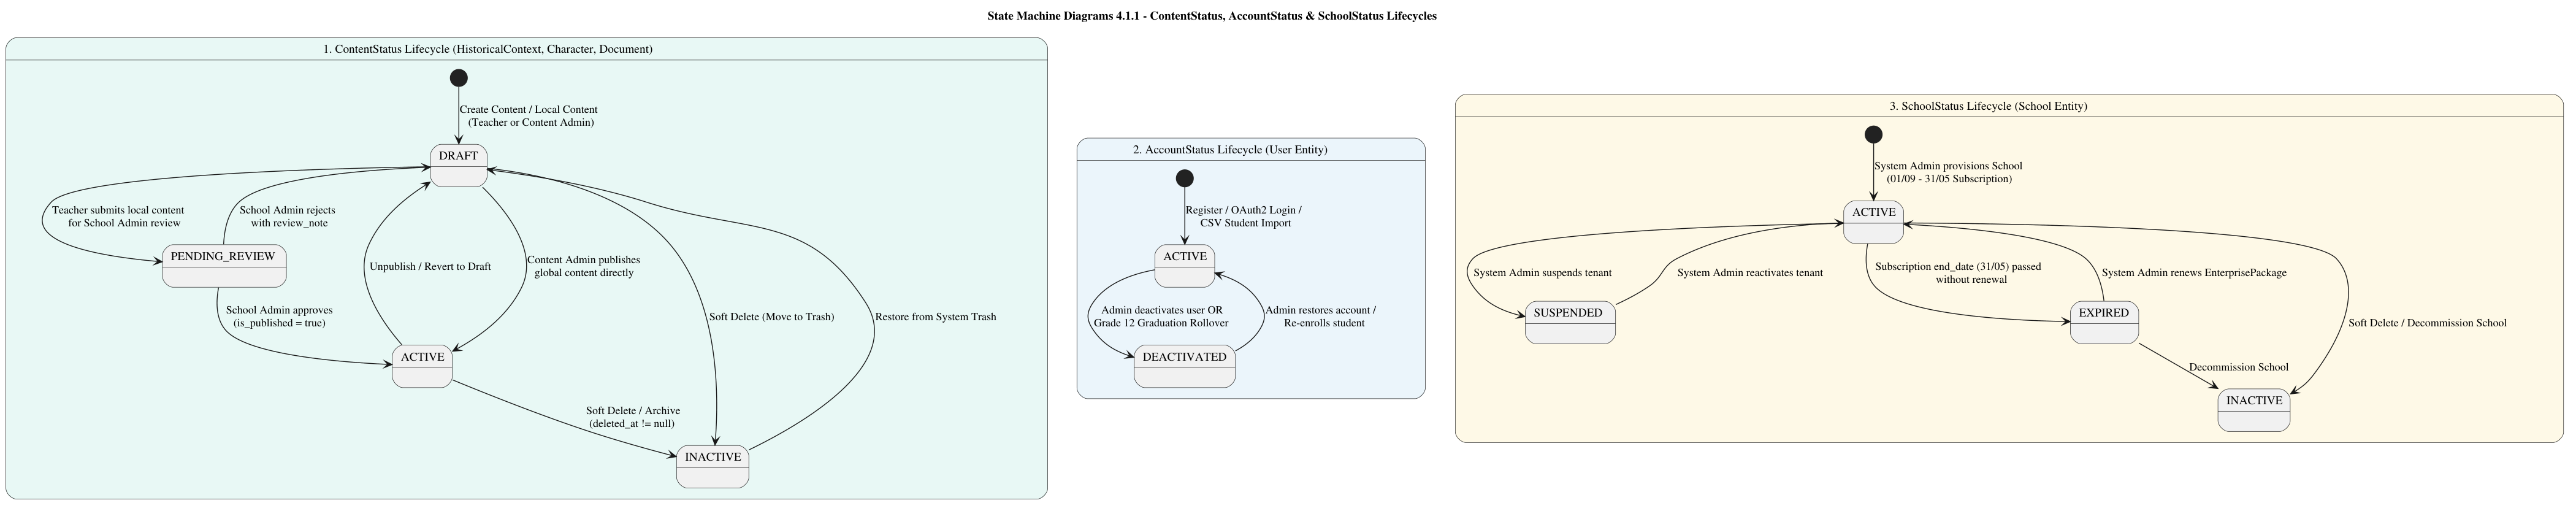
\includegraphics[width=0.98\textwidth,height=0.25\textheight,keepaspectratio]{figures/stm_01_content_and_account.png}
    \caption{State Machine Diagrams -- ContentStatus, AccountStatus and SchoolStatus Lifecycles}
    \label{fig:stm_01_content_and_account}
\end{figure}

\begin{figure}[htbp]
    \centering
    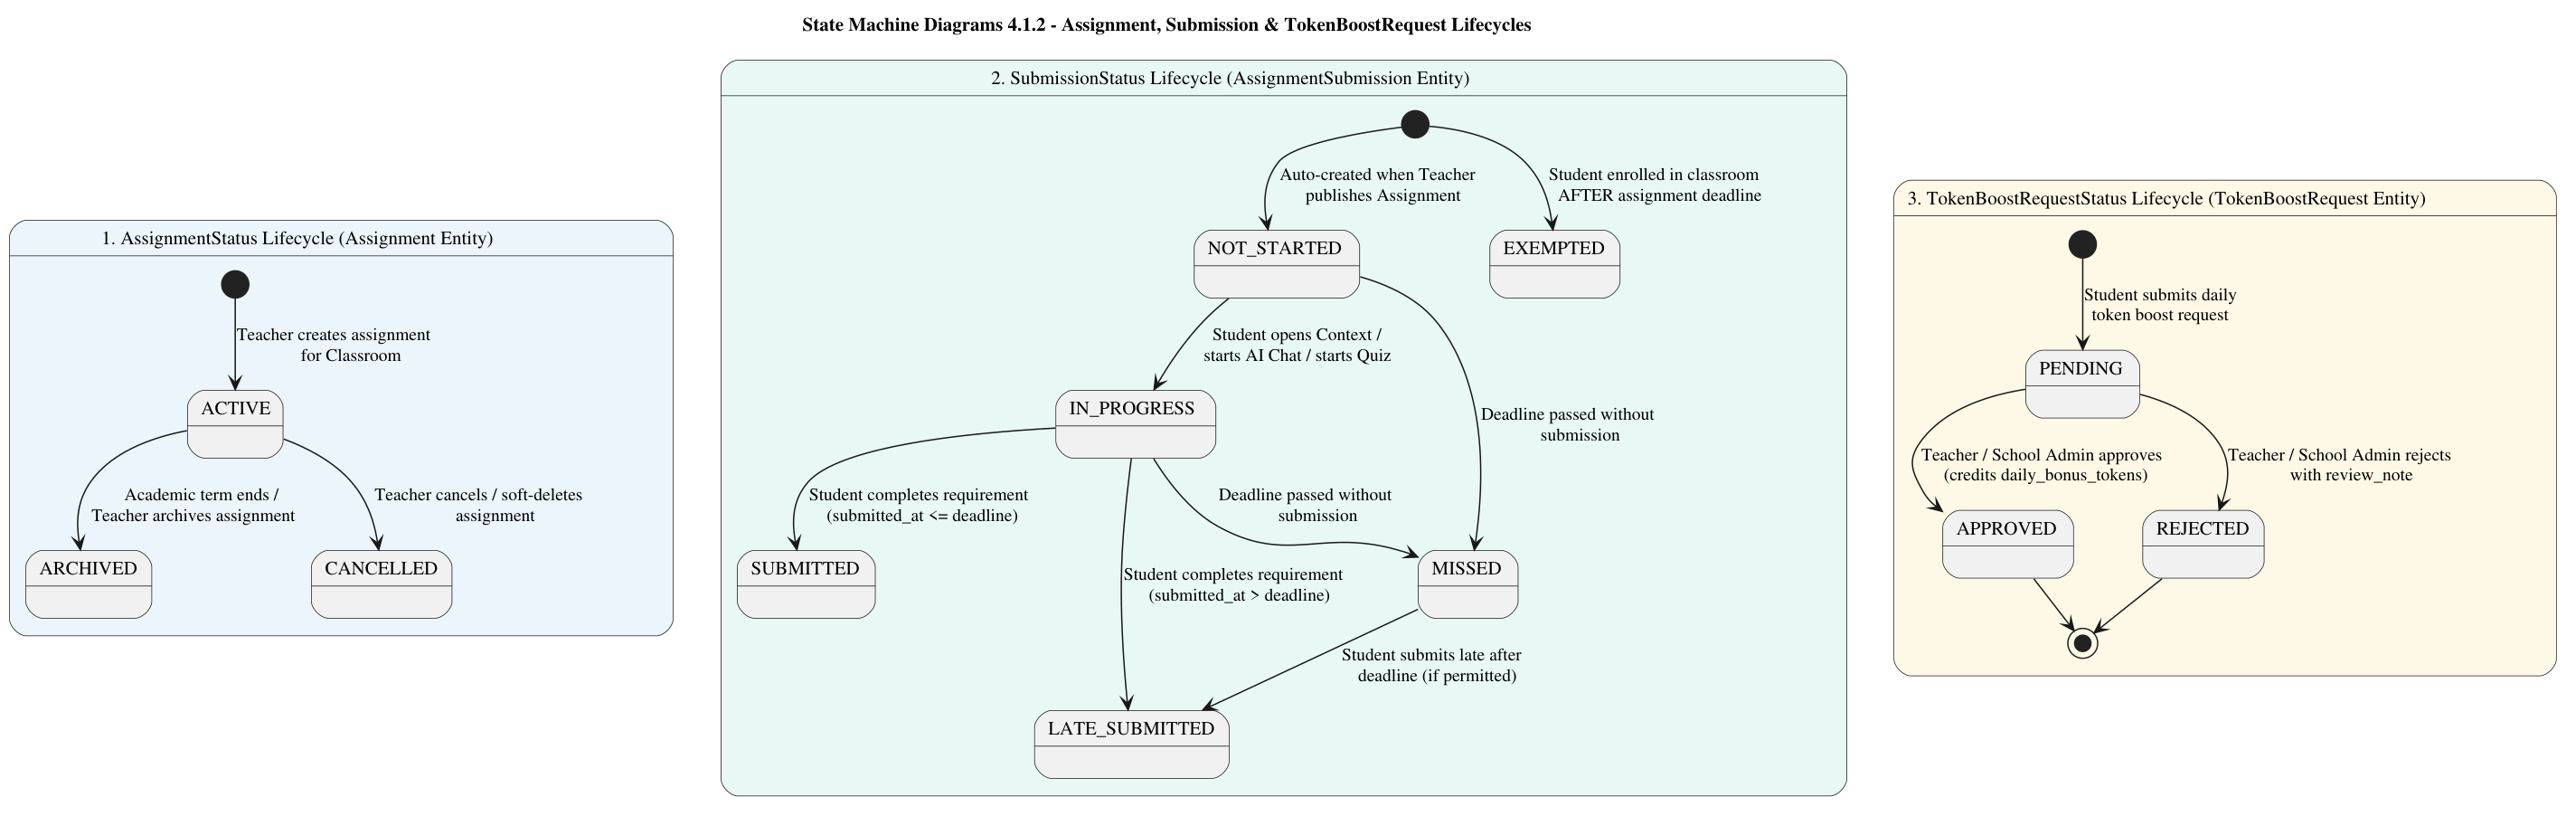
\includegraphics[width=0.98\textwidth,height=0.25\textheight,keepaspectratio]{figures/stm_02_assignment_and_token.png}
    \caption{State Machine Diagrams -- AssignmentStatus, SubmissionStatus and TokenBoostRequestStatus Lifecycles}
    \label{fig:stm_02_assignment_and_token}
\end{figure}

\begin{figure}[htbp]
    \centering
    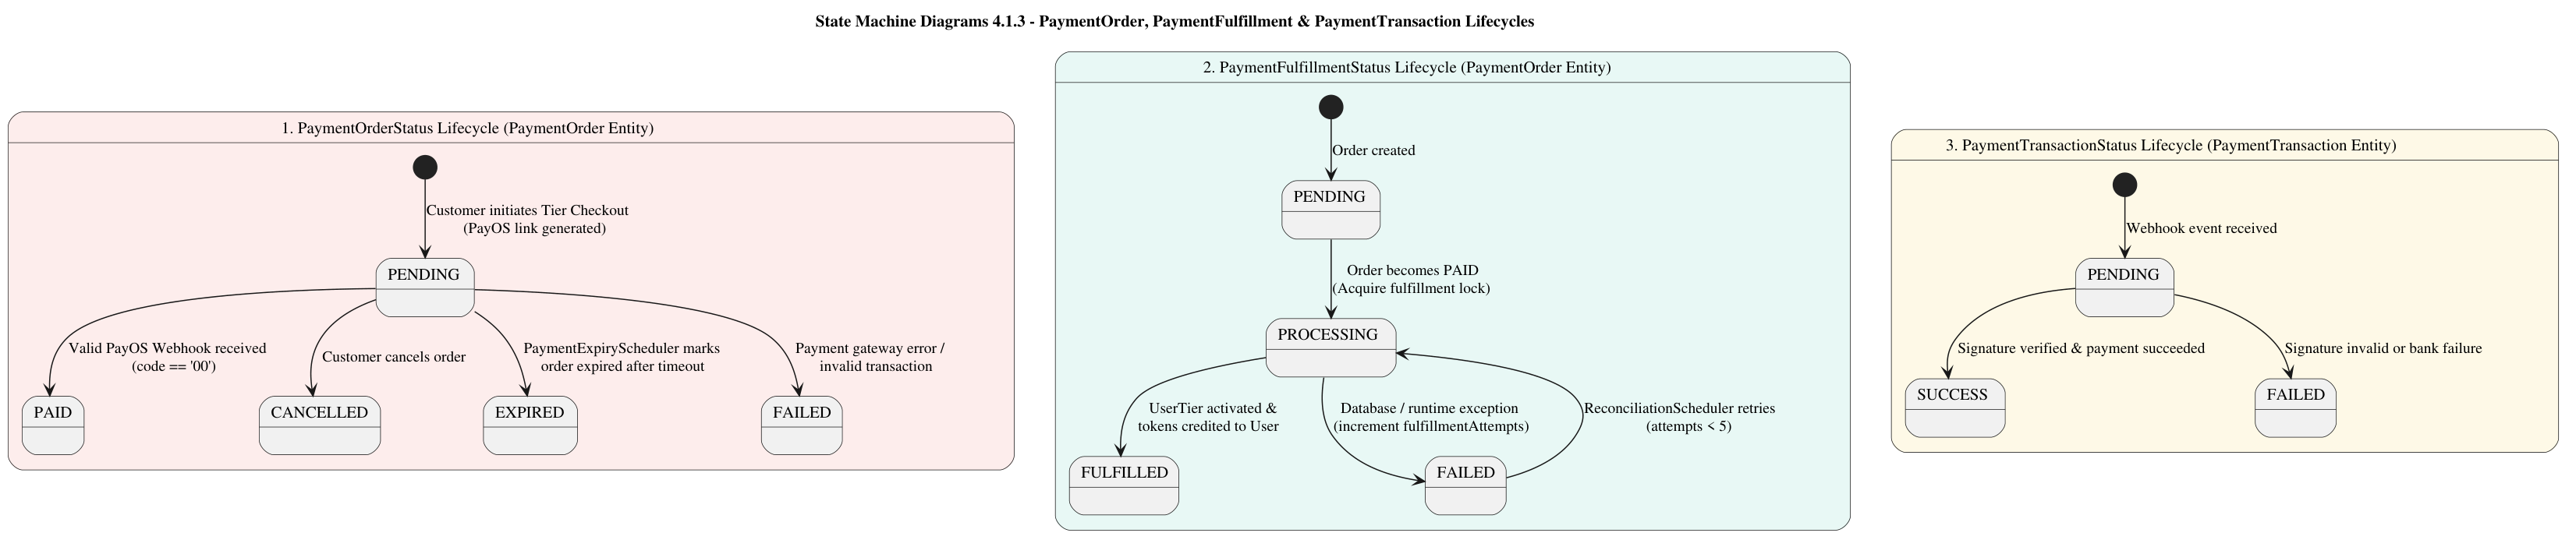
\includegraphics[width=0.98\textwidth,height=0.25\textheight,keepaspectratio]{figures/stm_03_payment_lifecycle.png}
    \caption{State Machine Diagrams -- PaymentOrderStatus, PaymentFulfillmentStatus and PaymentTransactionStatus Lifecycles}
    \label{fig:stm_03_payment_lifecycle}
\end{figure}

\paragraph{State Transition and Trigger Traceability Matrix}
Table~\ref{tab:state_transitions} maps each state enumeration in the system to its valid transitions and triggering API endpoints or schedulers.

\footnotesize
\begin{longtable}{|L{3.3cm}|L{2.6cm}|L{3.5cm}|L{4.7cm}|}
\hline
\rowcolor{tableheader}
\textbf{Entity / Enum} & \textbf{States} & \textbf{Valid Transitions} & \textbf{Triggering Feature / API / Scheduler} \\
\hline
\endhead
HistoricalContext, Character, Document\newline(ContentStatus) & DRAFT, PENDING\_\ab REVIEW, ACTIVE, INACTIVE & DRAFT $\rightarrow$ PENDING\_\ab REVIEW\newline PENDING\_\ab REVIEW $\rightarrow$ ACTIVE / DRAFT\newline DRAFT $\leftrightarrow$ ACTIVE\newline DRAFT/ACTIVE $\rightarrow$ INACTIVE\newline INACTIVE $\rightarrow$ DRAFT & Teacher submits local content (PUT /submit-review); School Admin approves or rejects (PUT /local-content/\ab \{id\}/status); Content Admin publishes, deletes, or restores (SystemTrash\ab Controller). \\
\hline
User\newline(AccountStatus) & ACTIVE, DEACTIVATED & ACTIVE $\leftrightarrow$ DEACTIVATED & Admin deactivates or restores user (AdminUser\ab Controller); End-of-year Grade 12 rollover (AcademicLifecycle\ab ServiceImpl). \\
\hline
School\newline(SchoolStatus) & ACTIVE, INACTIVE, SUSPENDED, EXPIRED & ACTIVE $\leftrightarrow$ SUSPENDED\newline ACTIVE $\leftrightarrow$ EXPIRED\newline ACTIVE/EXPIRED $\rightarrow$ INACTIVE & System Admin updates status or renews package (AdminSchool\ab Controller); Subscription expiry check after 31/05. \\
\hline
Assignment\newline(AssignmentStatus) & ACTIVE, CANCELLED, ARCHIVED & ACTIVE $\rightarrow$ ARCHIVED\newline ACTIVE $\rightarrow$ CANCELLED & Teacher creates, cancels, or archives classroom assignment (TeacherAssignment\ab Controller). \\
\hline
Assignment\ab Submission\newline(SubmissionStatus) & NOT\_STARTED, IN\_PROGRESS, SUBMITTED, LATE\_\ab SUBMITTED, MISSED, EXEMPTED & NOT\_STARTED $\rightarrow$ IN\_PROGRESS\newline IN\_PROGRESS $\rightarrow$ SUBMITTED / LATE\_\ab SUBMITTED\newline NOT\_STARTED/IN\_PROGRESS $\rightarrow$ MISSED\newline [*] $\rightarrow$ EXEMPTED & Student starts or submits assignment (StudentAssignment\ab Controller); Quiz and Chat sync hooks; Late student enrollment auto-exemption (ClassroomImport\ab Processor). \\
\hline
TokenBoostRequest\newline(TokenBoost\ab RequestStatus) & PENDING, APPROVED, REJECTED & PENDING $\rightarrow$ APPROVED\newline PENDING $\rightarrow$ REJECTED & Student requests boost (POST /token-boost-\ab requests); Teacher or School Admin reviews (PUT /token-boost-\ab requests/\ab \{id\}/review). \\
\hline
PaymentOrder\newline(PaymentOrder\ab Status) & PENDING, PAID, CANCELLED, EXPIRED, FAILED & PENDING $\rightarrow$ PAID / CANCELLED / EXPIRED / FAILED & PayOS Webhook (PayOSWebhook\ab Controller), User cancel (PaymentController), Expiry job (PaymentExpiry\ab Scheduler). \\
\hline
PaymentOrder\newline(PaymentFulfillment\ab Status) & PENDING, PROCESSING, FULFILLED, FAILED & PENDING $\rightarrow$ PROCESSING $\rightarrow$ FULFILLED / FAILED\newline FAILED $\rightarrow$ PROCESSING & PaymentFulfillment\ab Service and PaymentFulfillment\ab Reconciliation\ab Scheduler. \\
\hline
PaymentTransaction\newline(PaymentTransaction\ab Status) & PENDING, SUCCESS, FAILED & PENDING $\rightarrow$ SUCCESS / FAILED & Webhook verification in PaymentWebhook\ab Service. \\
\hline
\caption{Complete State Machine Traceability Matrix}
\label{tab:state_transitions}
\end{longtable}
\normalsize

\newpage
\subsection{Main Business Workflow Activity Diagrams}

HistoryTalk defines five end-to-end Main Business Workflows (WF-01 to WF-05), each owned by one team member in alignment with the Project Management Plan (Report 2 RACI Matrix), involving multiple actors and transitioning the state of core domain entities.

{\small
\begin{longtable}{|C{1.1cm}|L{3.2cm}|L{2.3cm}|L{2.5cm}|L{4.8cm}|}
\hline
\rowcolor{tableheader}
\textbf{ID} & \textbf{Workflow Name} & \textbf{Owner} & \textbf{Actors Involved} & \textbf{Primary Entities \& State Changes} \\
\hline
\endhead
WF-01 & B2B School Onboarding, Classroom Management \& Student Analytics & \vn{Trần Quốc Dinh}\newline(SE196495) & System Admin, School Admin, Teacher, School Student & School (ACTIVE), Classroom (ACTIVE), User (ACTIVE), ClassStudent, Assignment\ab Submission (EXEMPTED) \\
\hline
WF-02 & Global Content Management, PDF/OCR Document Ingestion \& Multi-Tenant Access & \vn{Võ Đồng Đức Khải}\newline(SE196405) & Content Admin, Teacher, School Admin & Historical\ab Context, Character, Document (DRAFT $\rightarrow$ PENDING\_\ab REVIEW $\rightarrow$ ACTIVE), VectorChunk \\
\hline
WF-03 & Grounded AI Historical Roleplay Chat, RAG Retrieval \& Token Quota Management & \vn{Nguyễn Minh Trí}\newline(SE192645) & School Student / Customer, Teacher, School Admin & ChatSession, Message, User (dailyTokens\ab Used), TokenBoost\ab Request (PENDING $\rightarrow$ APPROVED) \\
\hline
WF-04 & Timed Quiz Assessment Engine, Interactive Map \& PayOS Payment Fulfillment & \vn{Đỗ Quốc Bảo}\newline(SE193803) & Teacher, School Student, Customer, PayOS Gateway & Assignment (ACTIVE), QuizSession, QuizAnswer\ab Detail, PaymentOrder (PENDING $\rightarrow$ PAID, FULFILLED) \\
\hline
WF-05 & Frontend Client Interactive Learning Workflows, Classroom Submissions \& Daily Quests & \vn{Nguyễn Công Thành}\newline(SE196309) & School Student, Customer, Teacher & Assignment\ab Submission (NOT\_STARTED $\rightarrow$ IN\_PROGRESS $\rightarrow$ SUBMITTED), UserQuest\ab Progress (claimed), DailyCheckIn \\
\hline
\caption{Main Business Workflows Summary and Ownership Matrix}
\label{tab:main_workflows}
\end{longtable}
}

\begin{figure}[htbp]
    \centering
    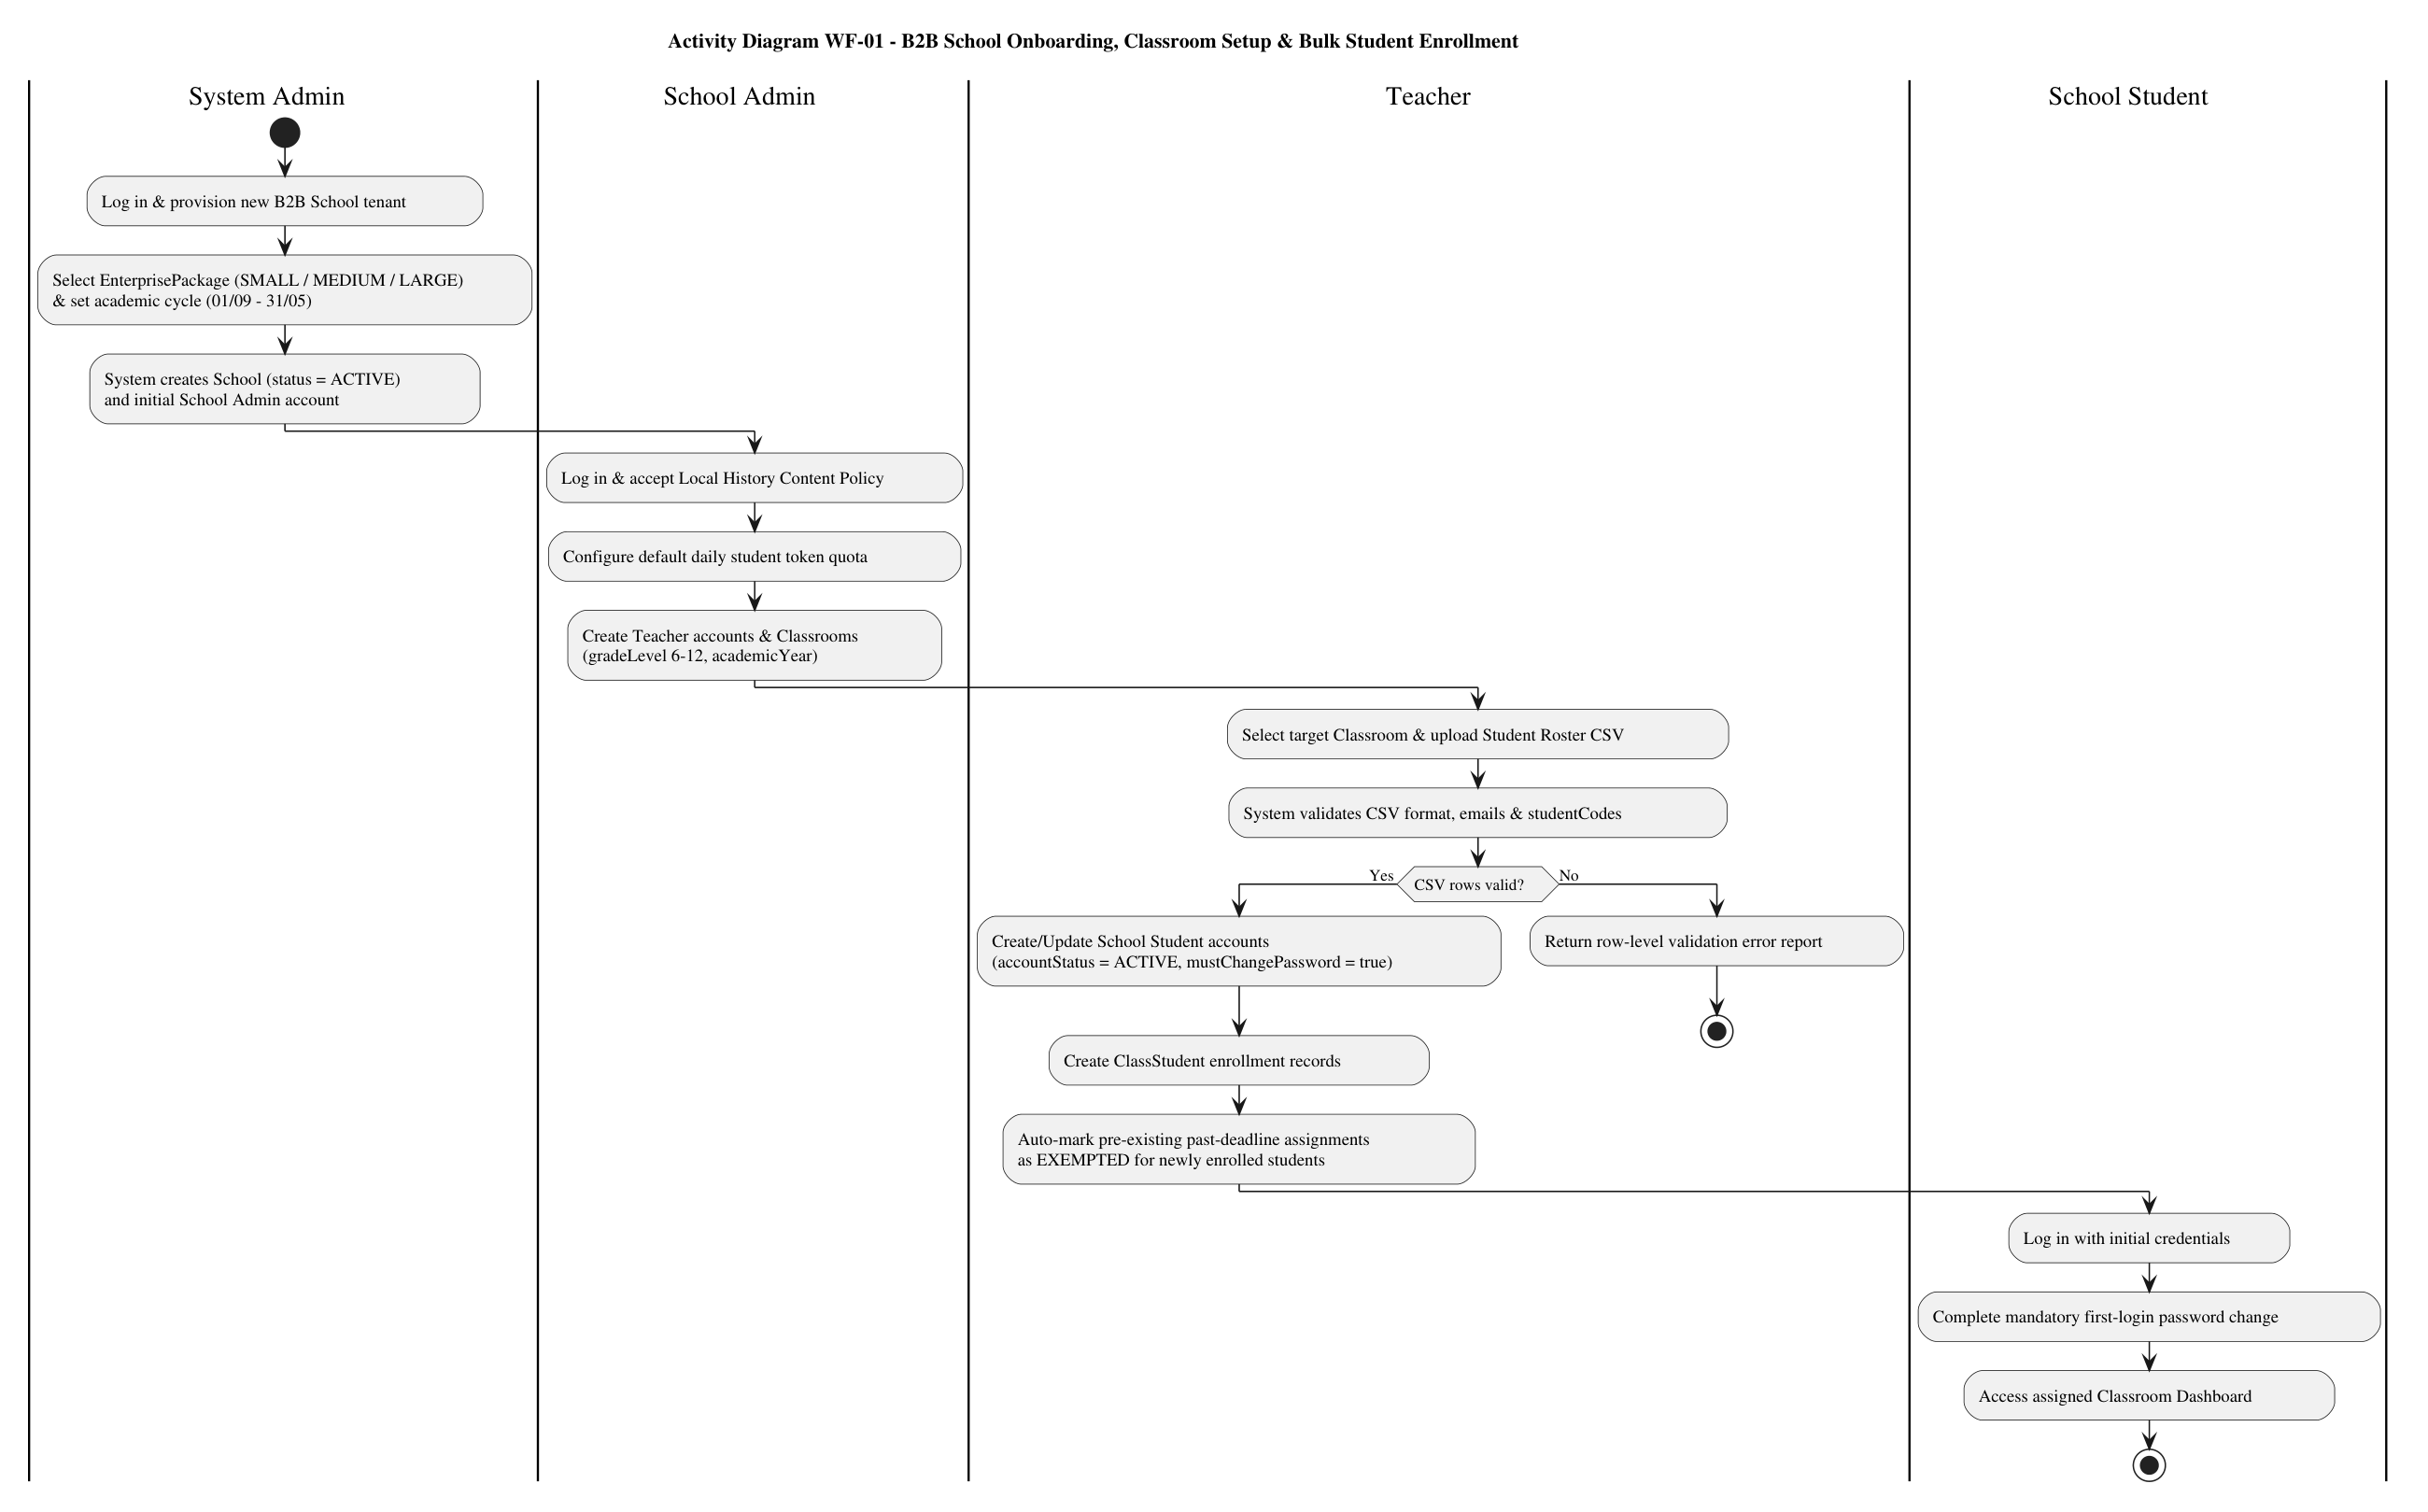
\includegraphics[width=0.95\textwidth,height=0.42\textheight,keepaspectratio]{figures/act_wf01_school_onboarding_and_enrollment.png}
    \caption{Activity Diagram WF-01 -- B2B School Onboarding, Classroom Setup and Bulk Student Enrollment}
    \label{fig:act_wf01}
\end{figure}

\begin{figure}[htbp]
    \centering
    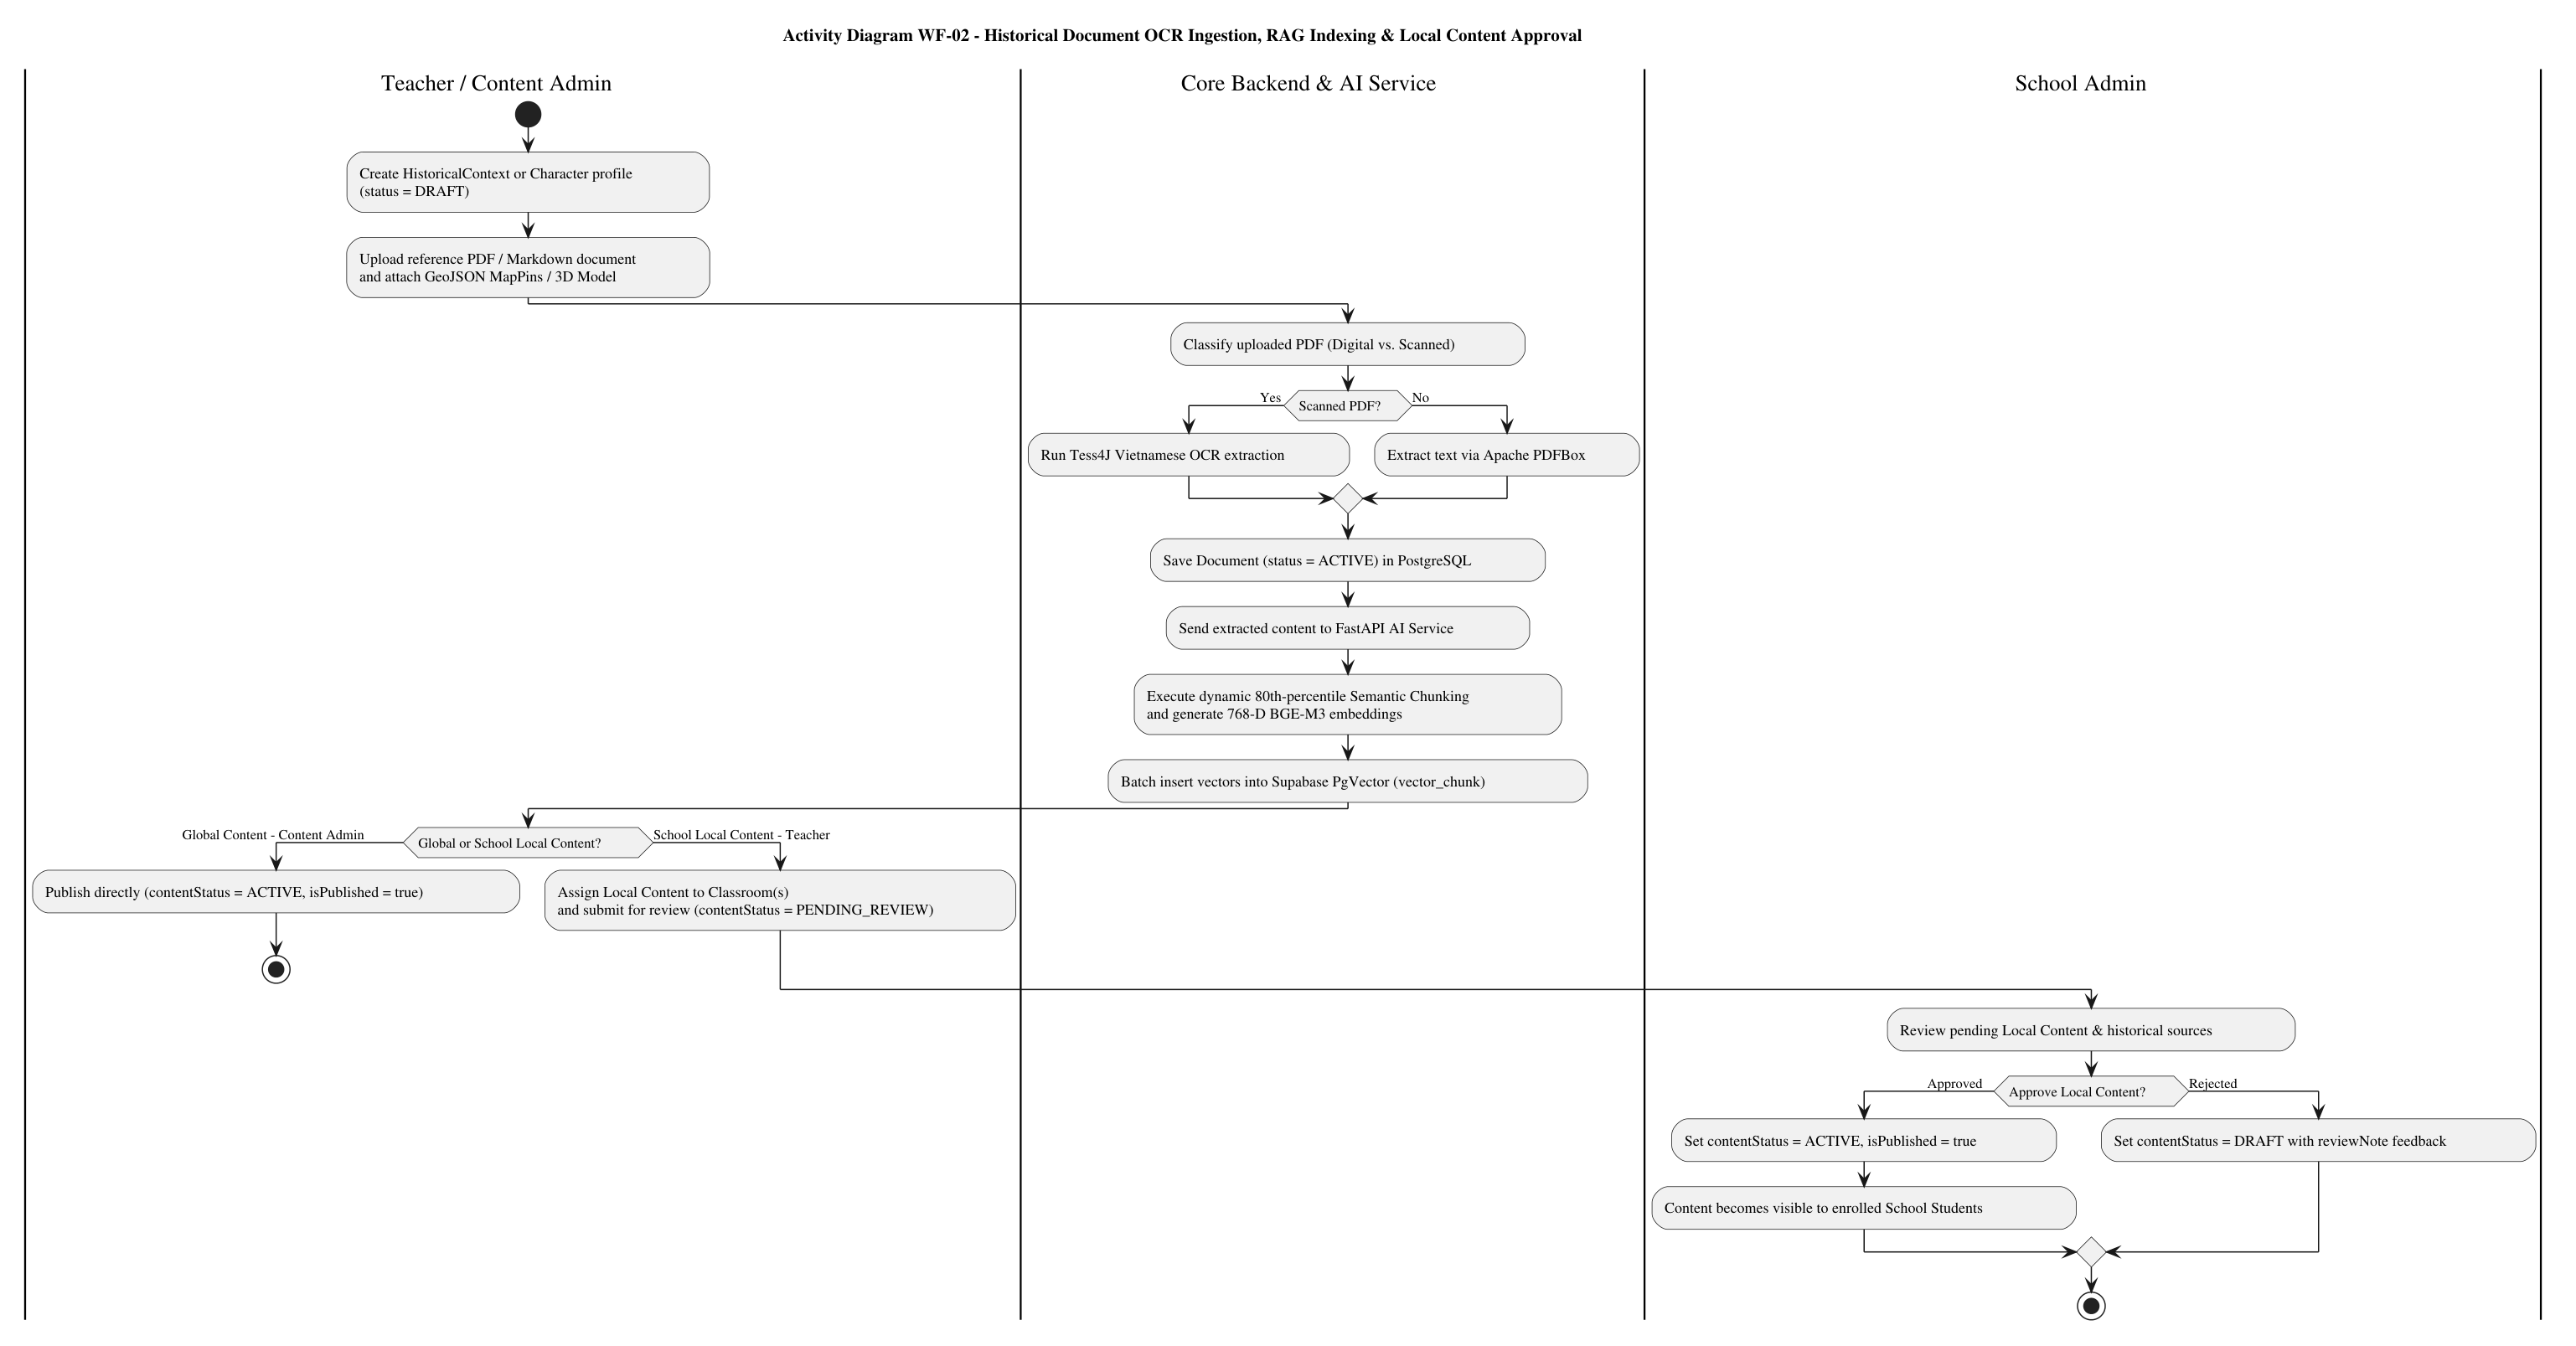
\includegraphics[width=0.95\textwidth,height=0.42\textheight,keepaspectratio]{figures/act_wf02_rag_content_and_local_approval.png}
    \caption{Activity Diagram WF-02 -- Historical Document OCR Ingestion, RAG Indexing and Content Approval}
    \label{fig:act_wf02}
\end{figure}

\begin{figure}[htbp]
    \centering
    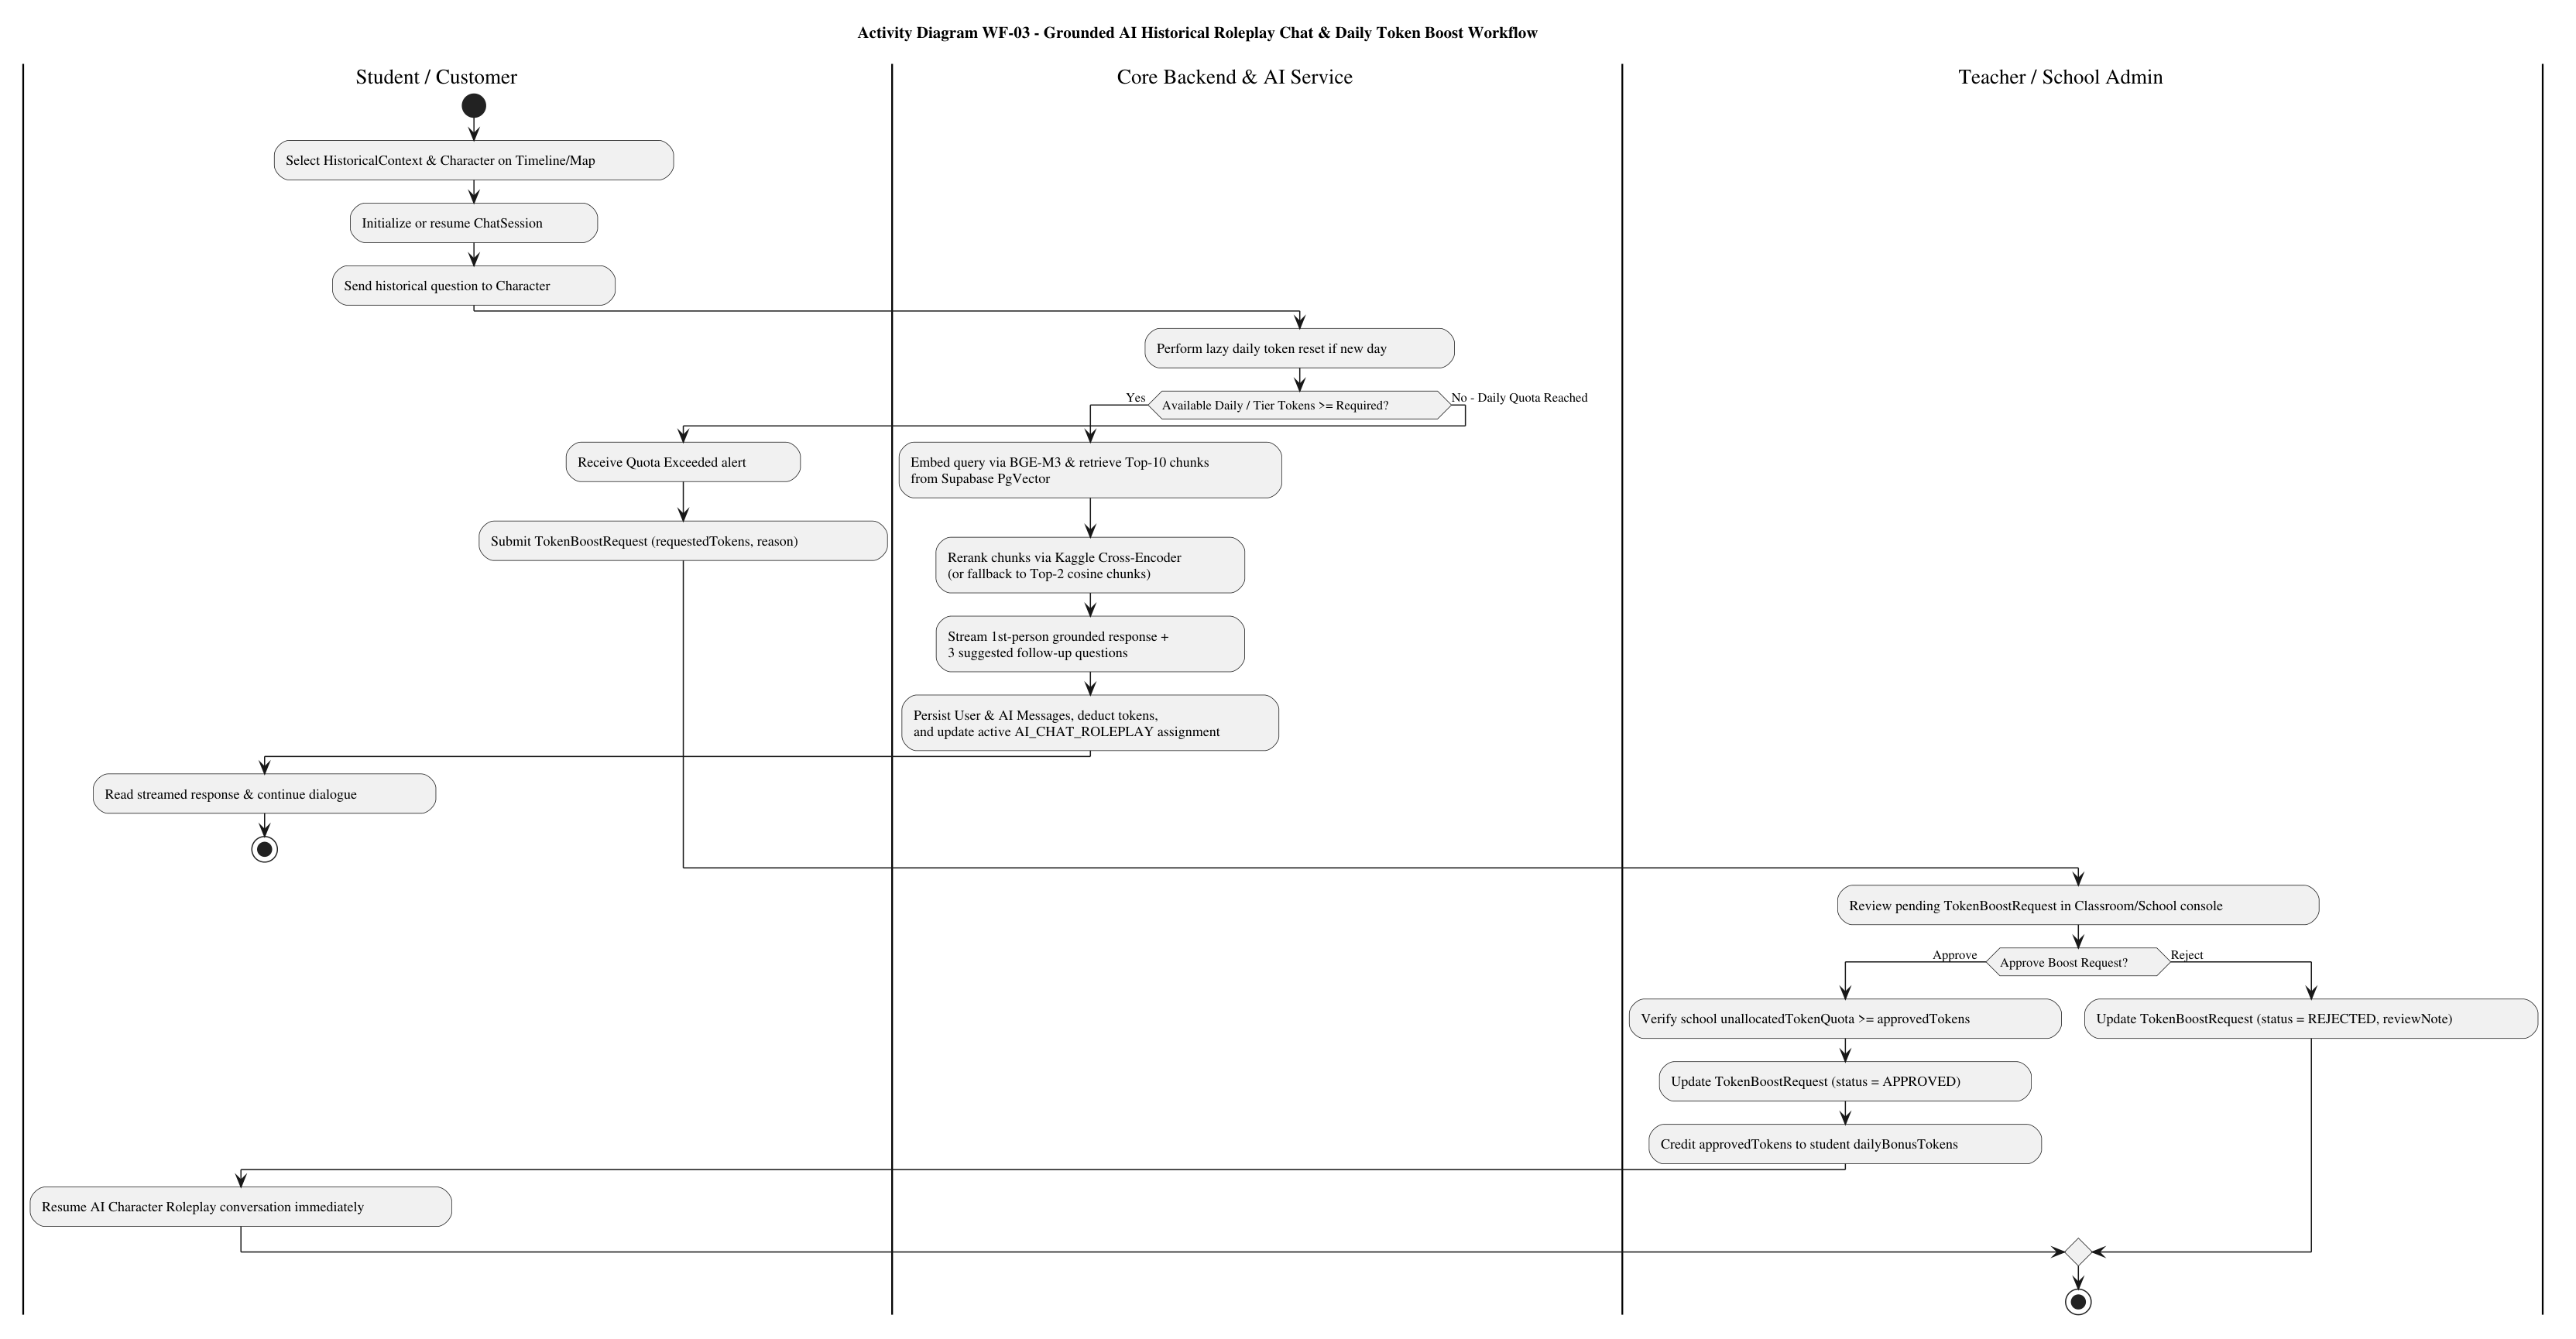
\includegraphics[width=0.95\textwidth,height=0.42\textheight,keepaspectratio]{figures/act_wf03_ai_character_roleplay_and_token_boost.png}
    \caption{Activity Diagram WF-03 -- Grounded AI Historical Roleplay Chat and Daily Token Boost Workflow}
    \label{fig:act_wf03}
\end{figure}

\begin{figure}[htbp]
    \centering
    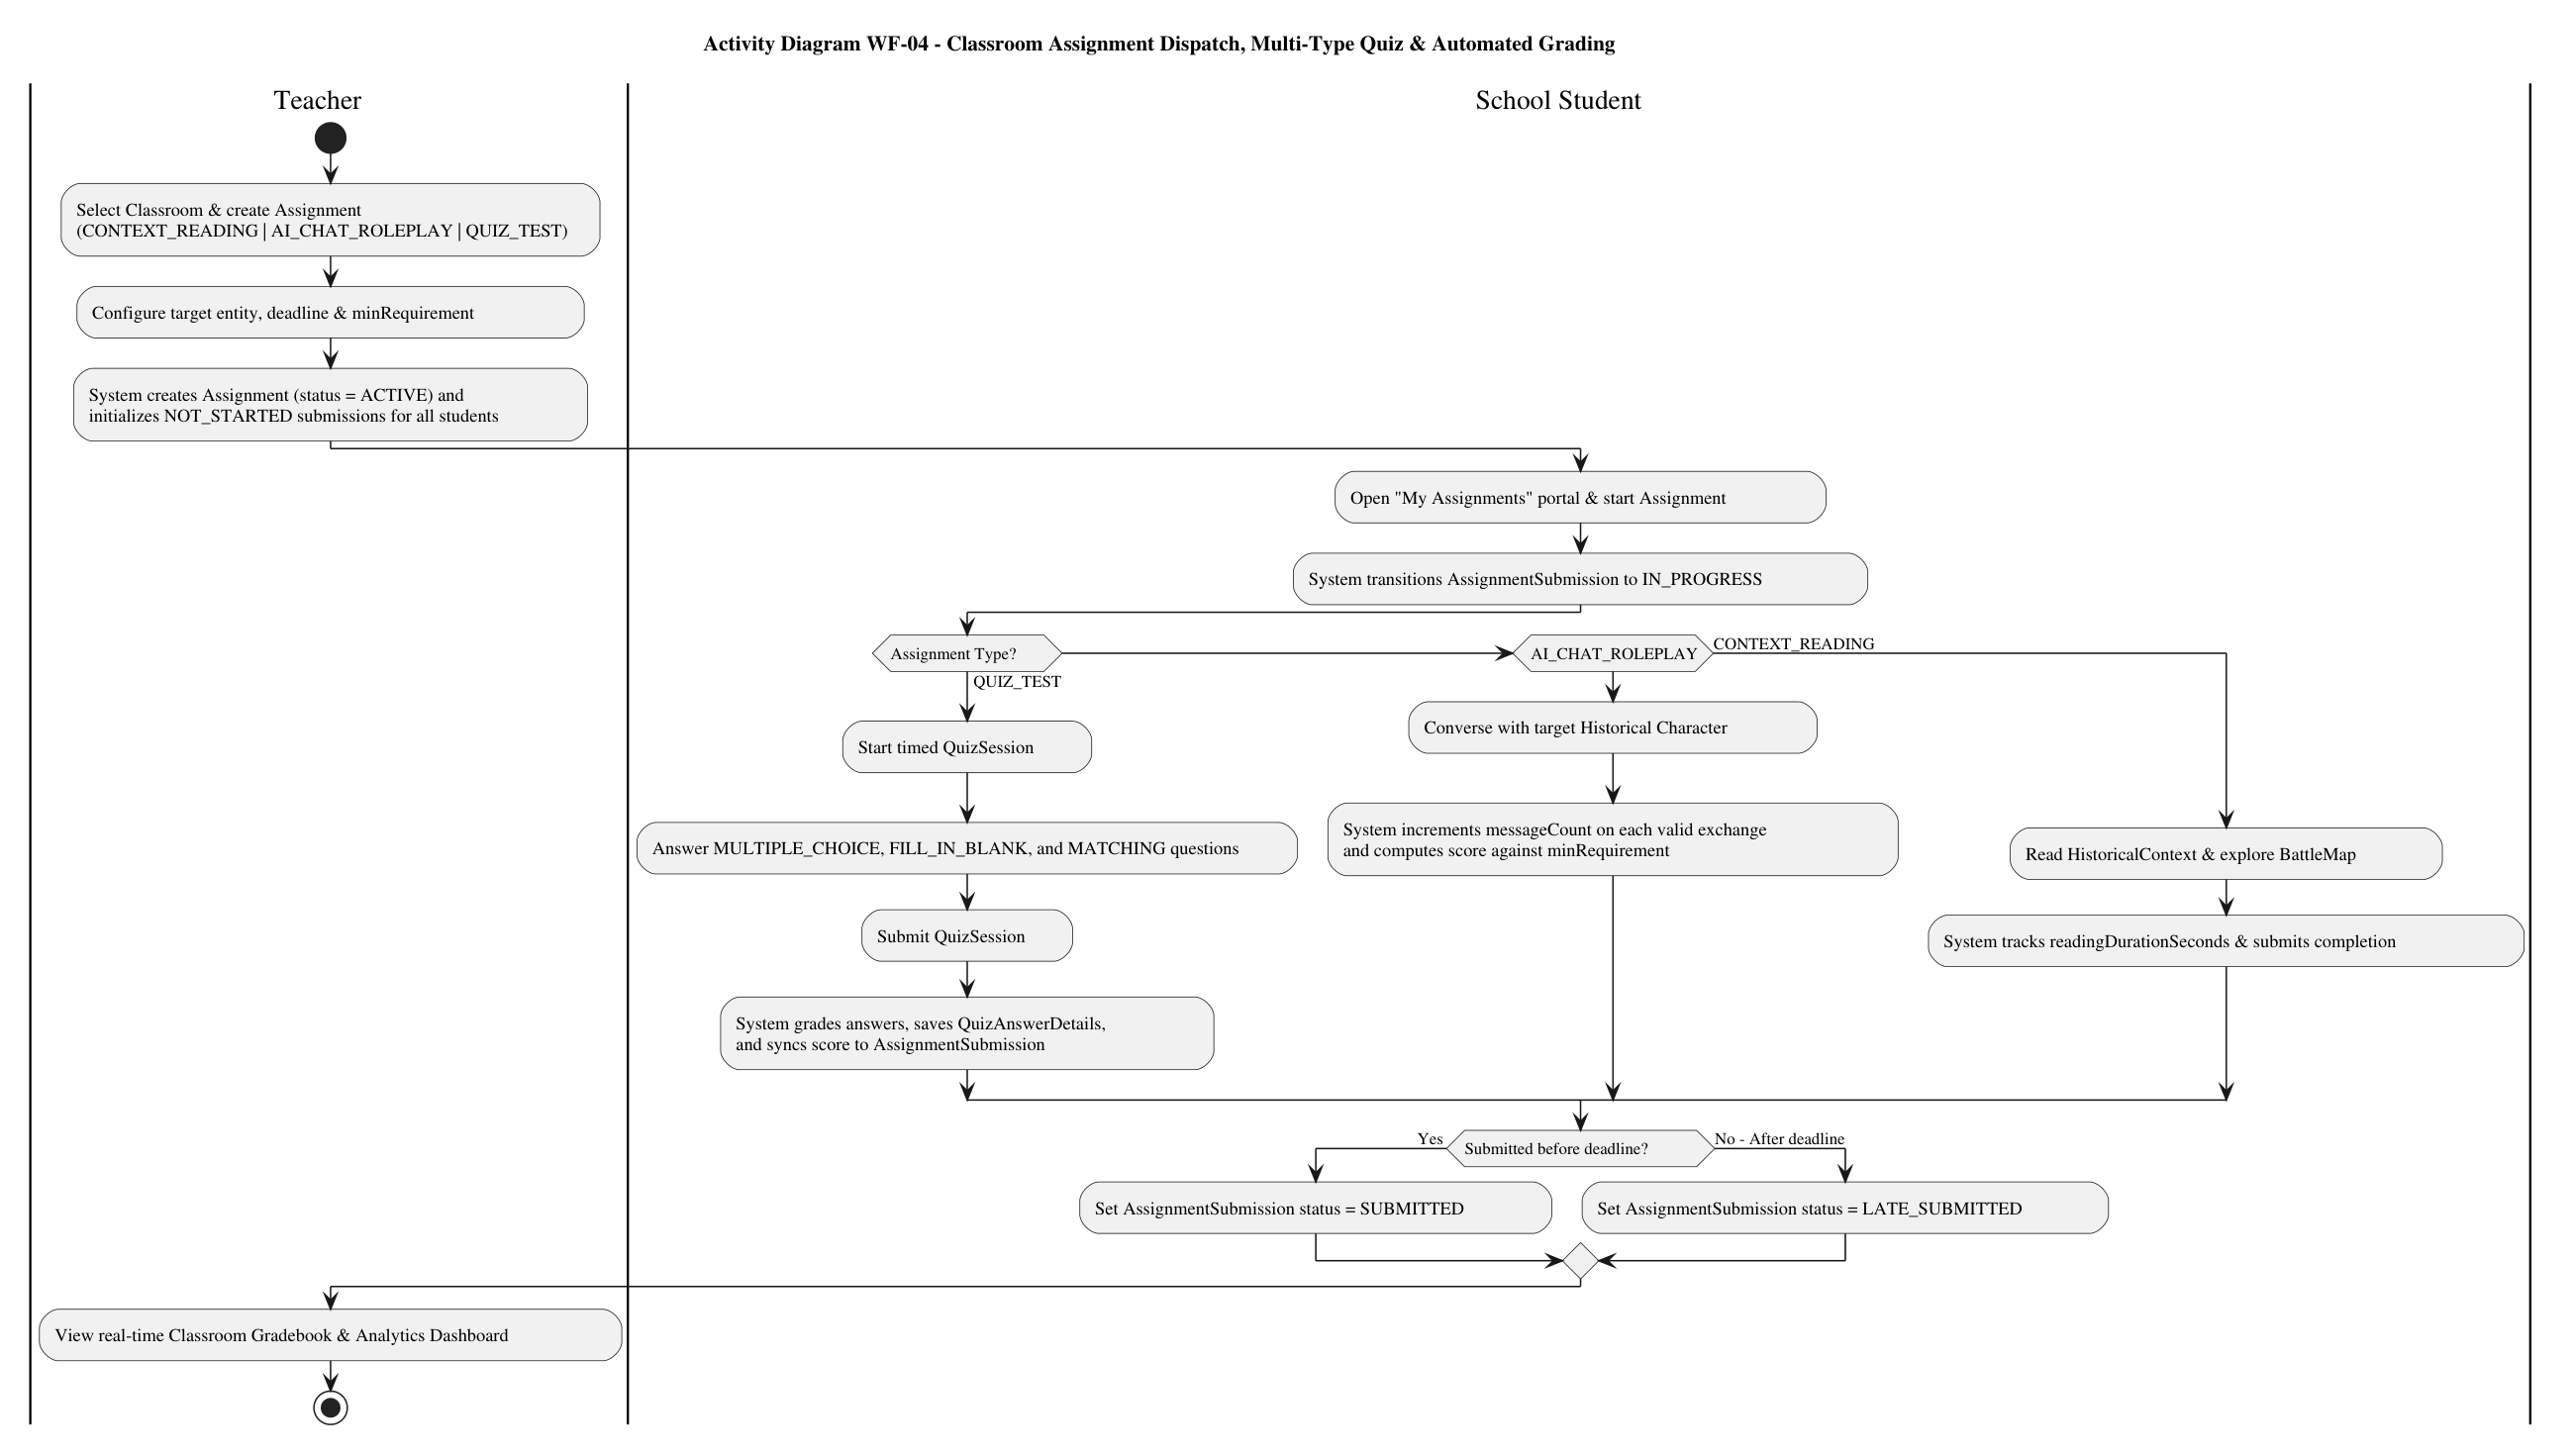
\includegraphics[width=0.95\textwidth,height=0.42\textheight,keepaspectratio]{figures/act_wf04_classroom_assignment_and_quiz_grading.png}
    \caption{Activity Diagram WF-04 -- Classroom Assignment Dispatch, Multi-Type Quiz and Automated Grading}
    \label{fig:act_wf04}
\end{figure}

\begin{figure}[htbp]
    \centering
    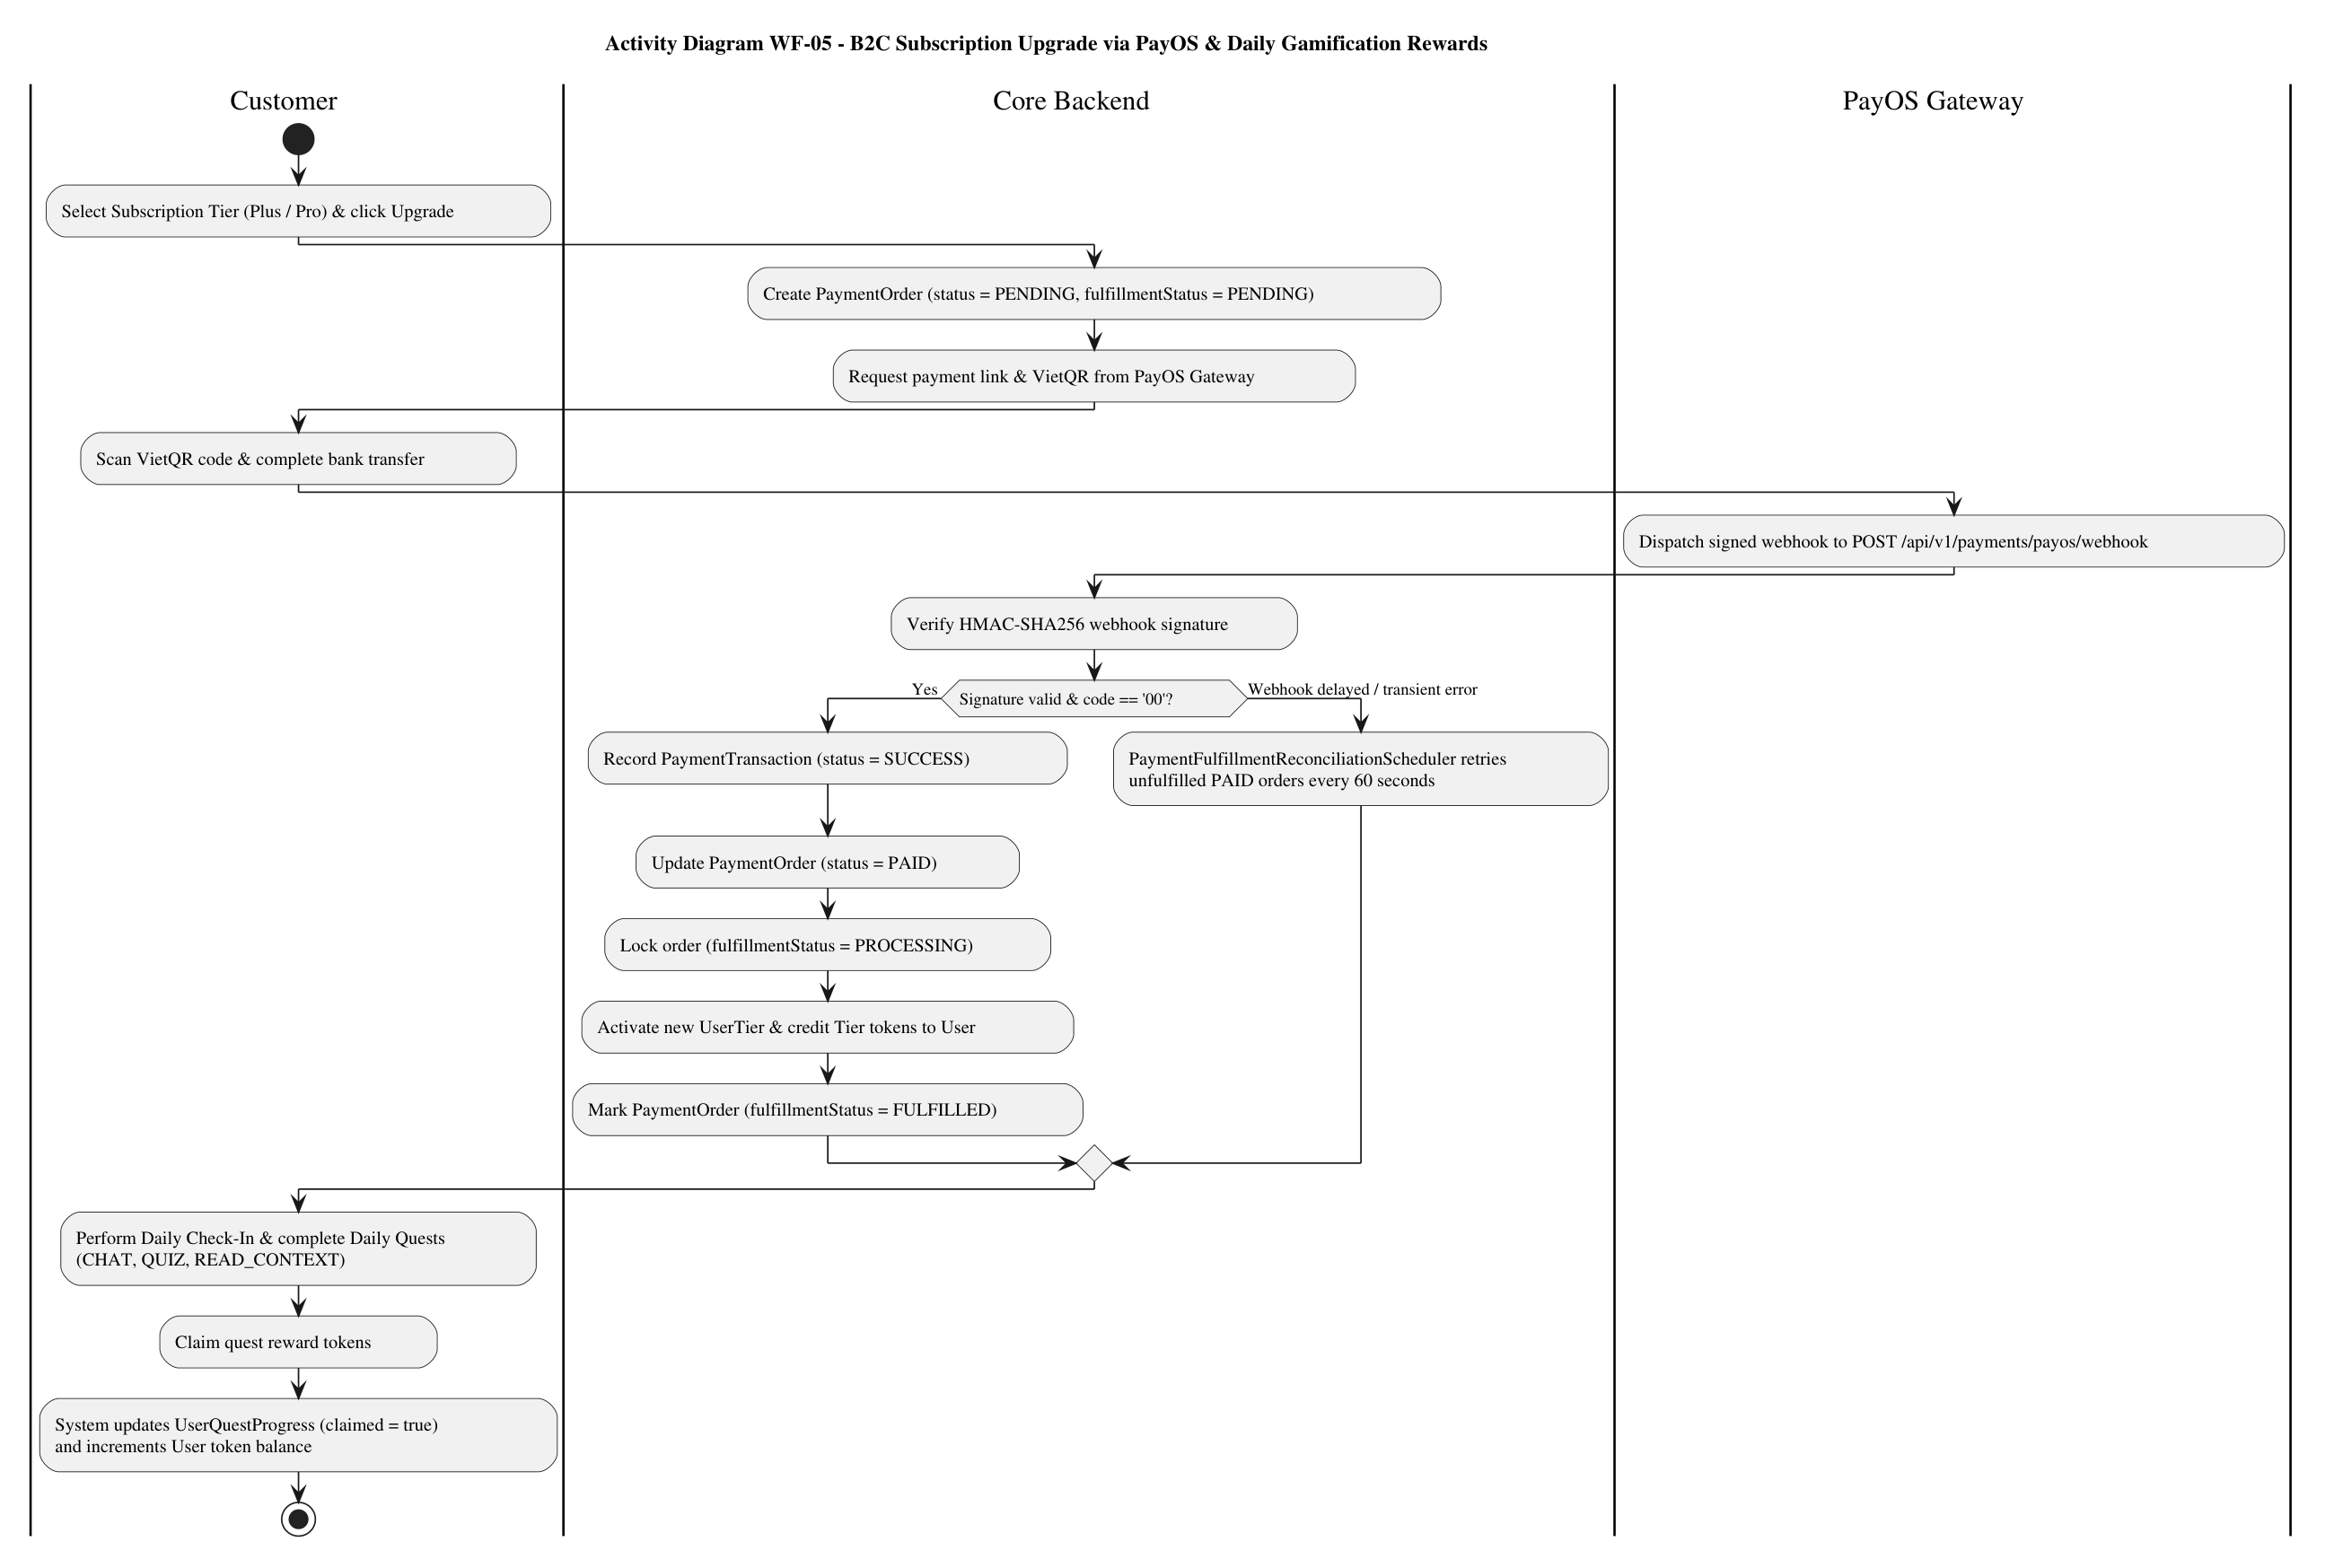
\includegraphics[width=0.95\textwidth,height=0.42\textheight,keepaspectratio]{figures/act_wf05_b2c_payos_subscription_and_gamification.png}
    \caption{Activity Diagram WF-05 -- B2C Subscription Upgrade via PayOS and Daily Gamification Rewards}
    \label{fig:act_wf05}
\end{figure}
